\documentclass[tikz, border=10pt]{standalone}

\usetikzlibrary{arrows}

\begin{document}
	
	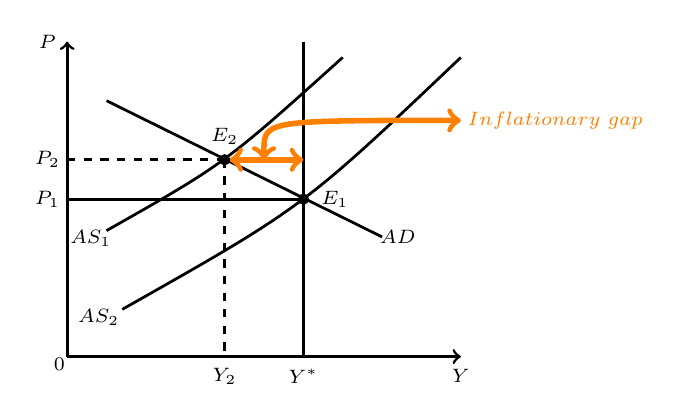
\begin{tikzpicture}[line width=1pt]
	\draw[->] (0, 0) -- (5, 0); % Горизонтальная линия
	\draw[->] (0, 0) -- (0, 4); % Вертикальная линия
	
	\draw (3, 0) -- (3, 4);
	\draw (0, 2) -- (3 ,2);
	\draw[dashed] (0, 2.5) -- (2, 2.5);
	\draw[dashed] (2, 2.5) -- (2, 0);
	\draw (0.5, 3.25) -- (4, 1.52);
	
	\draw (0.5, 1.6) .. controls (2, 2.45) and (2, 2.45) .. (3.5, 3.8);
	\draw (0.7, 0.6) .. controls (3, 1.9) and (3, 1.9) .. (5, 3.8);
	
	\draw[<->, color=orange, line width=2pt] (2.06, 2.5) -- (3, 2.5);
	\draw[<->, color=orange, line width=2pt] (2.5, 2.5) .. controls (2.5, 3) and (2.4, 3) .. (5, 3);
	
	\begin{scriptsize}
	\draw[fill=black]  (3, 2) circle (1.5pt);
	\draw[fill=black]  (2, 2.5) circle (1.5pt);
	
	\draw (-0.25, 4) node {$P$};
	\draw (-0.25, 2) node {$P_1$};
	\draw (-0.25, 2.5) node {$P_2$};
	
	\draw (3.4, 2) node {$E_1$};
	\draw (2, 2.8) node {$E_2$};
	
	\draw (5, -0.25) node {$Y$};
	\draw (3, -0.25) node {$Y^*$};
	\draw (2, -0.25) node {$Y_2$};
	
	\draw (-0.1, -0.1) node {$0$};
	
	\draw (4.2, 1.52) node {$AD$};
	\draw (0.3, 1.5) node {$AS_1$};
	\draw (0.4, 0.5) node {$AS_2$};
	
	\draw[color=orange] (6.2, 3) node {$Inflationary ~ gap$};
	\end{scriptsize}
	\end{tikzpicture}
\end{document}